\chapter{Word Embedding}
\cite{xing2015normalized}
\section{Monolingual Embedding}
\subsection{CBOW and Skip-gram Model}
	Word embeddings is distributed representation of words in a vector space. With the learning algorithm it can capture the contextual or co-occurrence information. The word embedding has an interesting and important property: similar words will have similar distribution in the embedding space, with that property, we can find meaningful near-synonyms or  Some successful methods for learning word embedding like word2vec  \cite{mikolov2013distributed}
	Continuous Bag-of-Words model(CBOW) and Skip-Gram model
	CBOW model and Skip-Gram model are currently the  common structures to learn the word embedding. Algorithmically,  CBOW tries to predict the current word based on the context while Skip-Gram model tries to maximize classification of a word based on another word in the same sentence.
	The neural probability language model defines the prediction probability using the softmax function:

	
	\begin{align}
	p(w_t | w_s) & = \textrm{softmax} {(s(w_t, w_s))} \\
	& = \frac{\exp\{s(w_t, w_s)\}}{\sum_{w^{\prime} \in W}{\exp\{s( w^{\prime}, w_s)\}}} 
	\end{align}
	where ${w_t}$ is target word)label word), ${w_s}$ is the source word(input word), for Skip-Gram model, the target word refers to the context words, the source word refers to the current word, for CBOW model is simply inverted. ${W}$ denotes the whole vocabulary. Then the training objective of the model is to maximize the log-likelihood on the training dataset, i.e. by maximizing:
	
	\begin{align}
	J_{ML} & = \log p(w_t| w_s)	\\
	& = s(w_t, w_s) - \log(\sum_{w^\prime \in W} {\exp\{s(w^\prime, w_s)\}})	
	\end{align}


	
	However the normalization on the whole vocabulary is very expensive because it is conducted for all words at every training step. The problem of predicting words can be considered as an independent binary classification task. For example in the Skip-Gram model, we consider all the context words as positive samples and the words randomly sampled from the dictionary as the negative ones. Then the training objective is 
	\[J_{NEG} = \log {Q_{\theta}{(D=1 | w^{\prime}, w_s)}} + \sum_{w^{\prime} \sim W} {\log{Q_{\theta}{(D=0 | w^{\prime}, w_s )}}}  \]
	
	where ${Q_{\theta}{(D=1| w^{\prime} w_s)}}$ is the binary logistic regression probability. In practice, we draw k contrastive words from the noise distribution. Since we only calculate the loss function for k samples instead the whole vocabulary, it becomes much faster to train.
	
	
	\[\frac{1}{T} \sum_{t=1}^{T} \sum_{-c<j<c, j\neq 0}{\textrm{log}{p(w_{t+j}|w_t)}}\]
	where c is the size of training context, larger context size make the results more precise at the cost of training time. Suppose we are give a scoring function to evaluate the word pair(word, context), the Skip-Gram model
	
	\[\frac{1}{T} \sum_{t=1}^{T} \sum_{-c<j<c, j\neq 0}{\textrm{log}{p(w_{t}|w_{t+j})}}\]
	 According to  empirical results, CBOW works better on smaller datasets because CBOW smoothes over a lot of the distributional information while Skip-Gram model performs better when we have larger datasets
	
	
	Noise-Contrastive Training
	
	
	\subsection{fastText}
	The training methods above treat each word as a distinct word embedding, however intuitively we can obtain more information from the morphological information of words. A subword model was proposed to try to fix such problem.The training network is similar, the model design a new presentation of the word: it adds speicial symbols $<$, ${>}$ as boundary information at the beginning and the end of a word. Then a normal word is represented as a bag of character $n$-grams . For example the word "where" and n equals 3, the it can be represented as the following 5 tri-grams: 
	\[ <wh, whe, her, ere, re>\]
	Suppose in this way we denote a word ${w}$ as ${G_{w}}$ the set of character ${n}$-grams, we assign for each character ${n}$-gram $g$ in ${G_{w}}$, we assign a distinct vector $z_g$, we will finally represent the embedding of word ${w}$ as the sum of these vector and also for the scoring function:
	\[s(w, w_s) = \sum_{g \in G_{w}} z_g^{T} w_s \]
	
\section{Supervised Learning of Cross-lingual Word Embedding}



	Cross-lingual word embedding is defined as word embedding of multiple languages in a joint embedding space. Mikolov first notice that the embedding distributions exhibit similar structure across languages. They proposed to use a linear mapping from the source embedding to target embedding. \\
	\begin{figure}[t]
		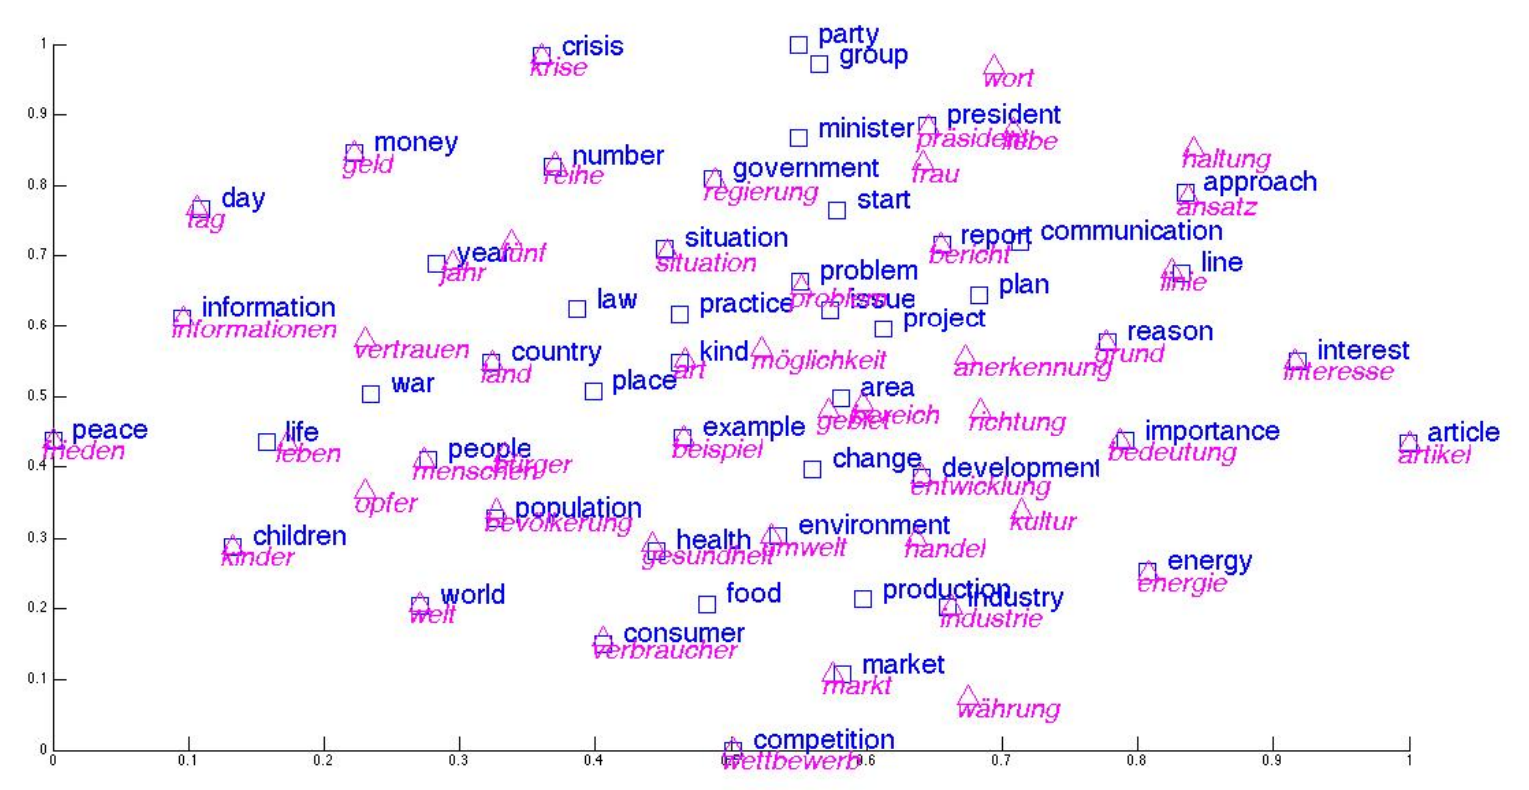
\includegraphics[width=14cm]{crossembedding}
		\centering
		\caption{A cross-lingual embedding space between German and English (\cite{ruder2017survey})}
	\end{figure}
	
	

	In the thesis, I assume there are two set of embeddings ${e}$, ${f}$trained separately on monolingual data.  The propose of cross-lingual word embedding training is to learn such a mapping ${W \in }$ from source embedding space to target embedding space, so $Wf_i, e_j$ in the same embedding space and for all corresponding word pairs, we need to optimize the mapping ${W}$, so that" 
	\[ \arg\min_{W \in R^{d \times d}} \sum_{i} \lVert Wf_i - e_i \rVert \]
	where $d$ is the dimension of embeddings, and the distance ${\lVert Wf_i - e_i \rVert}$ can be different types. We prefer the Euclidean distance.  

first observe that word embeddings trained separately on monolingual corpora exhibits isomorphic structure across languages, as illustrated in Figure {}. That means we can create a connection between source embedding and target embedding even with simple linear mapping. This has far-reaching implication on low-resource scenarios {}{}{}, because word embedding requires only plain text to train, which is the most abundant form of linguistic resource.
	

\subsection{***}
According to the training method we can divide the supervised method into three:
\begin{enumerate}
	\item Mapping based approaches\\
	First train the monolingual word embedding separately and then seek the seed dictionary to learn the mapping. 
	\item Pseudo-multi-lingual corpora-based approaches\\
	Use the monolingual embedding training method on constructed corpora that contains both the source and the target language.
	\item Joint methods\\
	Take the parallel text as input and minimize the source and target language losses jointly with the cross-lingual regularization term
\end{enumerate}

A dictionary is necessary for learning the cross-lingual word embedding. 
minimizing the distance in a bilingual dictionary.\\

Xing \cite{ } showed that the results are improved when we constrain the ${W}$ to be an orthogonal matrix. This constraint,  the optimal transformation can be efficiently calculated in linear time with respect to the vocabulary size.

The problem then is simplified as the Procrustes problem and there exists a closed-form solution obtained from the SVD of ${EF^T}$

\subsection{Orthogonal Constraints}
Starting from \cite{mikolov2013exploiting}, the mapping from source embedding space to target embedding space can be represented as a linear repression. The objective can be defined as:
\[ \min_{W} \sum_{i} {\lvert Wf - e  \rVert}^2 \]
Since we retrieve the word translation according to cosine similarity, it's better to solve the problem by redefine the optimization function using the cosine distance:
\[ \argmax{W} {\sum_{i} (W f_i)^T e^i} \]. We consider the source and target embedding in the same space. In this case, the normalization constraint on word vectors can be satisfied by constraining $W$ as an orthogonal matrix. 
This is equivalent to minimizing the (squared) Frobenius norm of the residual matrix:
\[ W^* = \argmin{W} {\lVert WF - E \rVert}^2_F \]
The problem boils down to the Procrustes problem which has a closed form solution obtained from the singular value decomposition (SVD).
\[W* = = UV^T , \quad U\Sigma V^T = SVD(EF^T) \]
\subsection{CSLS Loss}
Inspired from the work of \cite{conneau2017word}, where the dictionary inducted from CSLS loss: ${\bm{e}}$
\[ CSLS(\bm{e} ,\bm{f}) = -2 cos(\bm{e}, \bm{f}) + \frac{1}{k} \sum_{\bm{e}^{\prime} \in N_{\bm{e}}(\bm{f})} {cos(\bm{e}^{\prime}, \bm{f})}+ \frac{1}{k}  \sum_{\bm{f}^{\prime} \in N_{\bm{f}}(\bm{e})   } {cos(\bm{f}^{\prime}, \bm{e})}\]
since we have ${cos(\bm{We}, \bm{f}) = \bm{e}^T \bm{W}^T \bm{f}}$

The loss function can be rewritten as:
\[ \min_{\bm{W} \in } = \frac{1}{n} \sum_{i=1}^{n} \]


Minimization of a non-smooth cost function over the manifold of orthogonal matrices . Instead of using manifold optimization tools, \cite{bibid} proposed to derive convex relaxations that can lead to a simple and tractable minimization algorithm.
\begin{itemize}
	\item Spectral norm:
	replacing the set of orthogonal matrices $1$ by its convex hull, that is the set of matrices with singular values smaller than 1, the unit ball of the spectral norm 
	\item Frobenius norm:
	replacing the the set of orthogonal matrices $1$ with ball of radium $\sqrt{d}$ in Frobenius norm
\end{itemize}
 
With such two relaxations, the CSLS loss is constrained to a convex function with respect to the mapping $\bm{W}$.

We train the linear mapping with in the spectral norm by projected gradient descent:$2$ 
For each iteration, train the mapping $\bm{W}$ with gradient descent, then constrain the mapping by projection of the set.
\begin{itemize}
	\item Spectral norm\\
	take the SVD of the trained matrix, threshold the singular values to one
	\item Probenius norm\\
	divide the matrix by its Frobenius norm
\end{itemize} 



	
	